%%%% fatec-article.tex, 2024/03/10

\documentclass[
  a4paper,%% Tamanho de papel: a4paper, letterpaper (^), etc.
  12pt,%% Tamanho de fonte: 10pt (^), 11pt, 12pt, etc.
  english,%% Idioma secundário (penúltimo) (>)
  brazilian,%% Idioma primário (último) (>)
]{article}

%% Pacotes utilizados
\usepackage[]{fatec-article}

%% Início do documento
\begin{document}
\vspace{8cm}
\begin{center}
    \large \textbf{\title{ARTEFATOS DO PROJETO DE SOFTWARE}}
\end{center}

\maketitle

\break

\tableofcontents

\break


%exemplo da forma de organização das seções e subseções, você deverá adaptar o template para a realidade do seu projeto.

\section*{Diagramas UML}
    Nesta seção serão apresentados os diagramas da UML utilizados para a modelagem do sistema desenvolvido. Dentre os diagramas utilizados, pode-se citar: Diagrama de Caso de Uso, Diagrama de Classe e Diagrama de Objetos.
    
    \subsection*{Diagrama de Caso de Uso}
    \addcontentsline{toc}{section}{Diagrama de Caso de Uso}

            \begin{figure}[h]
\centering
\caption{Diagrama de caso de uso}%
\label{fig:diagrama-caso-uso}
 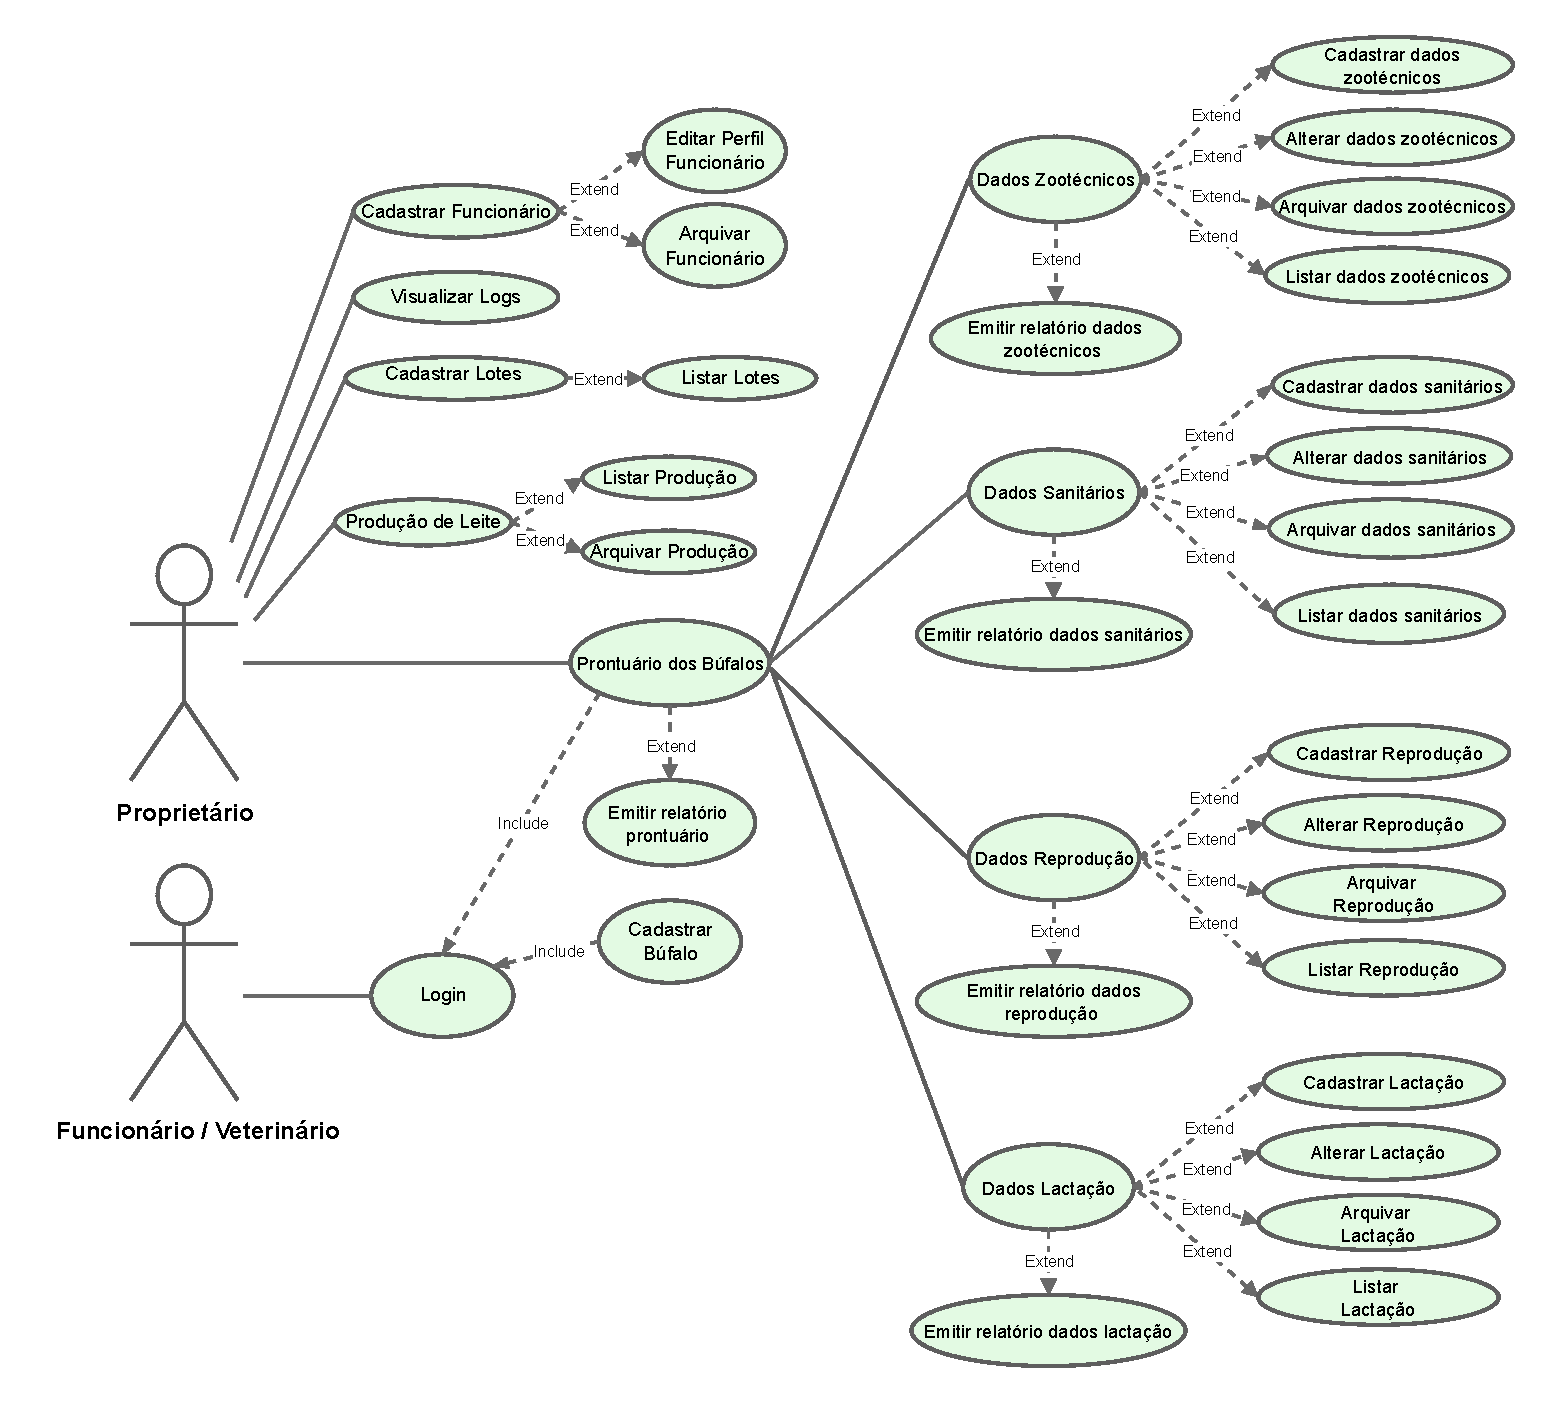
\includegraphics[width=0.9\textwidth]{Logos/CasosUso.pdf}
\SourceOrNote{Propria Autoria (2025)}
\end{figure}

    De acordo com o avanço do projeto, o diagrama de Caso de uso pode ser alterado.
    \newpage
    \subsection*{Diagrama de Classe}
    \addcontentsline{toc}{section}{Diagrama de Classe}


    \begin{figure}[h]
\centering
\caption{Diagrama de classe}%
\label{fig:diagrama-classe}
 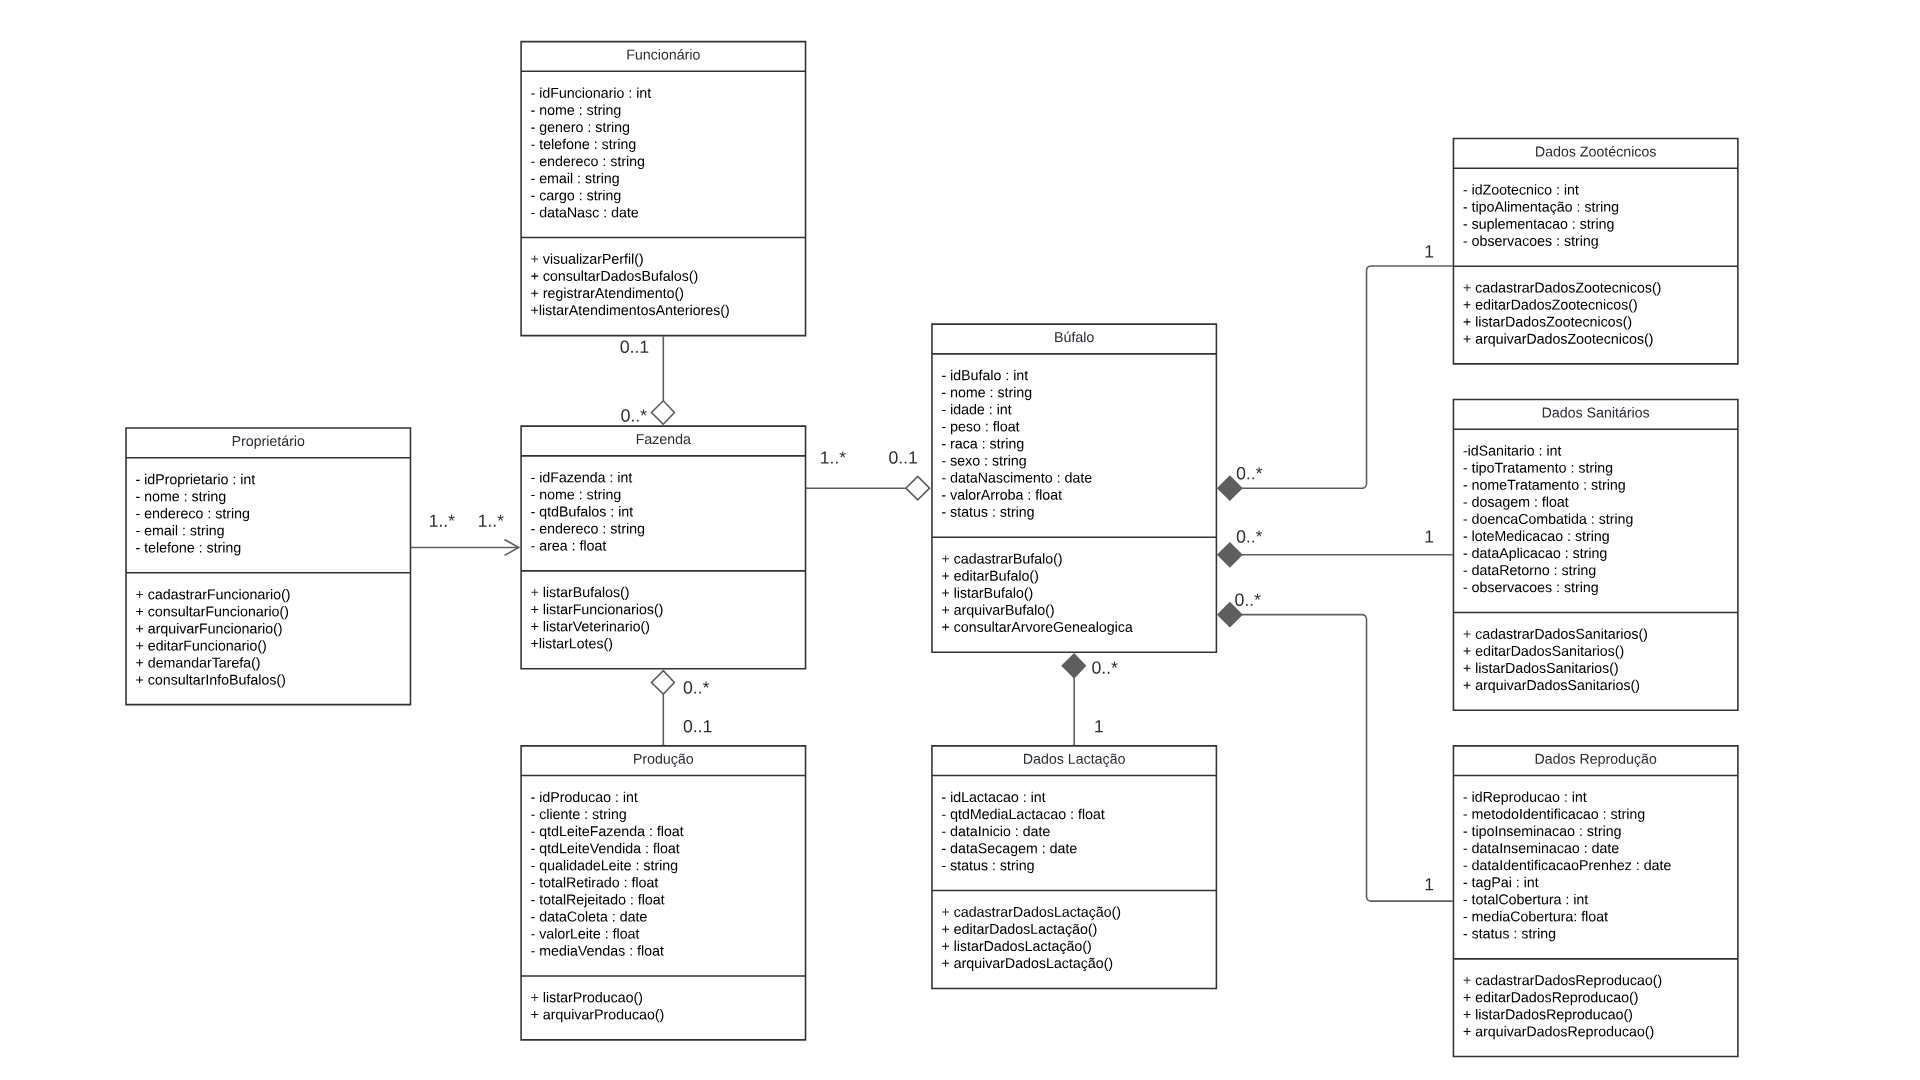
\includegraphics[width=1.2\textwidth]{Logos/CasosClasse.png}
\SourceOrNote{Propria Autoria (2025)}
\end{figure}

De acordo com o avanço do projeto, o diagrama Classe pode ser alterado.

\newpage
    \subsection*{Diagrama de Objetos}
    \addcontentsline{toc}{section}{Diagrama de Objetos}

        \begin{figure}[h]
\centering
\caption{Diagrama de objetos}%
\label{fig:diagrama-objetos}
 \includegraphics[width=1.1\textwidth]{Logos/CasosObjeto.png}
\SourceOrNote{Propria Autoria (2025)}
\end{figure}

De acordo com o avanço do projeto, o diagrama de O  bjeto pode ser alterado.
\newpage
\section*{Modelo Conceitual Banco de dados}
Nesta seção é apresentado o modelo conceitual do banco de dados, desenvolvido com base na identificação das entidades, relacionamentos e cardinalidades. Esse modelo tem como objetivo representar, de forma abstrata e independente de implementação, a estrutura geral das informações que compõem o sistema.
\subsection*{Modelo Conceitual Banco de dados}
 \addcontentsline{toc}{section}{Modelo Conceitual Banco de dados}

     \begin{figure}[h]
\centering
\caption{Modelo Banco de dados}%
\label{fig:modelo-conceitual}
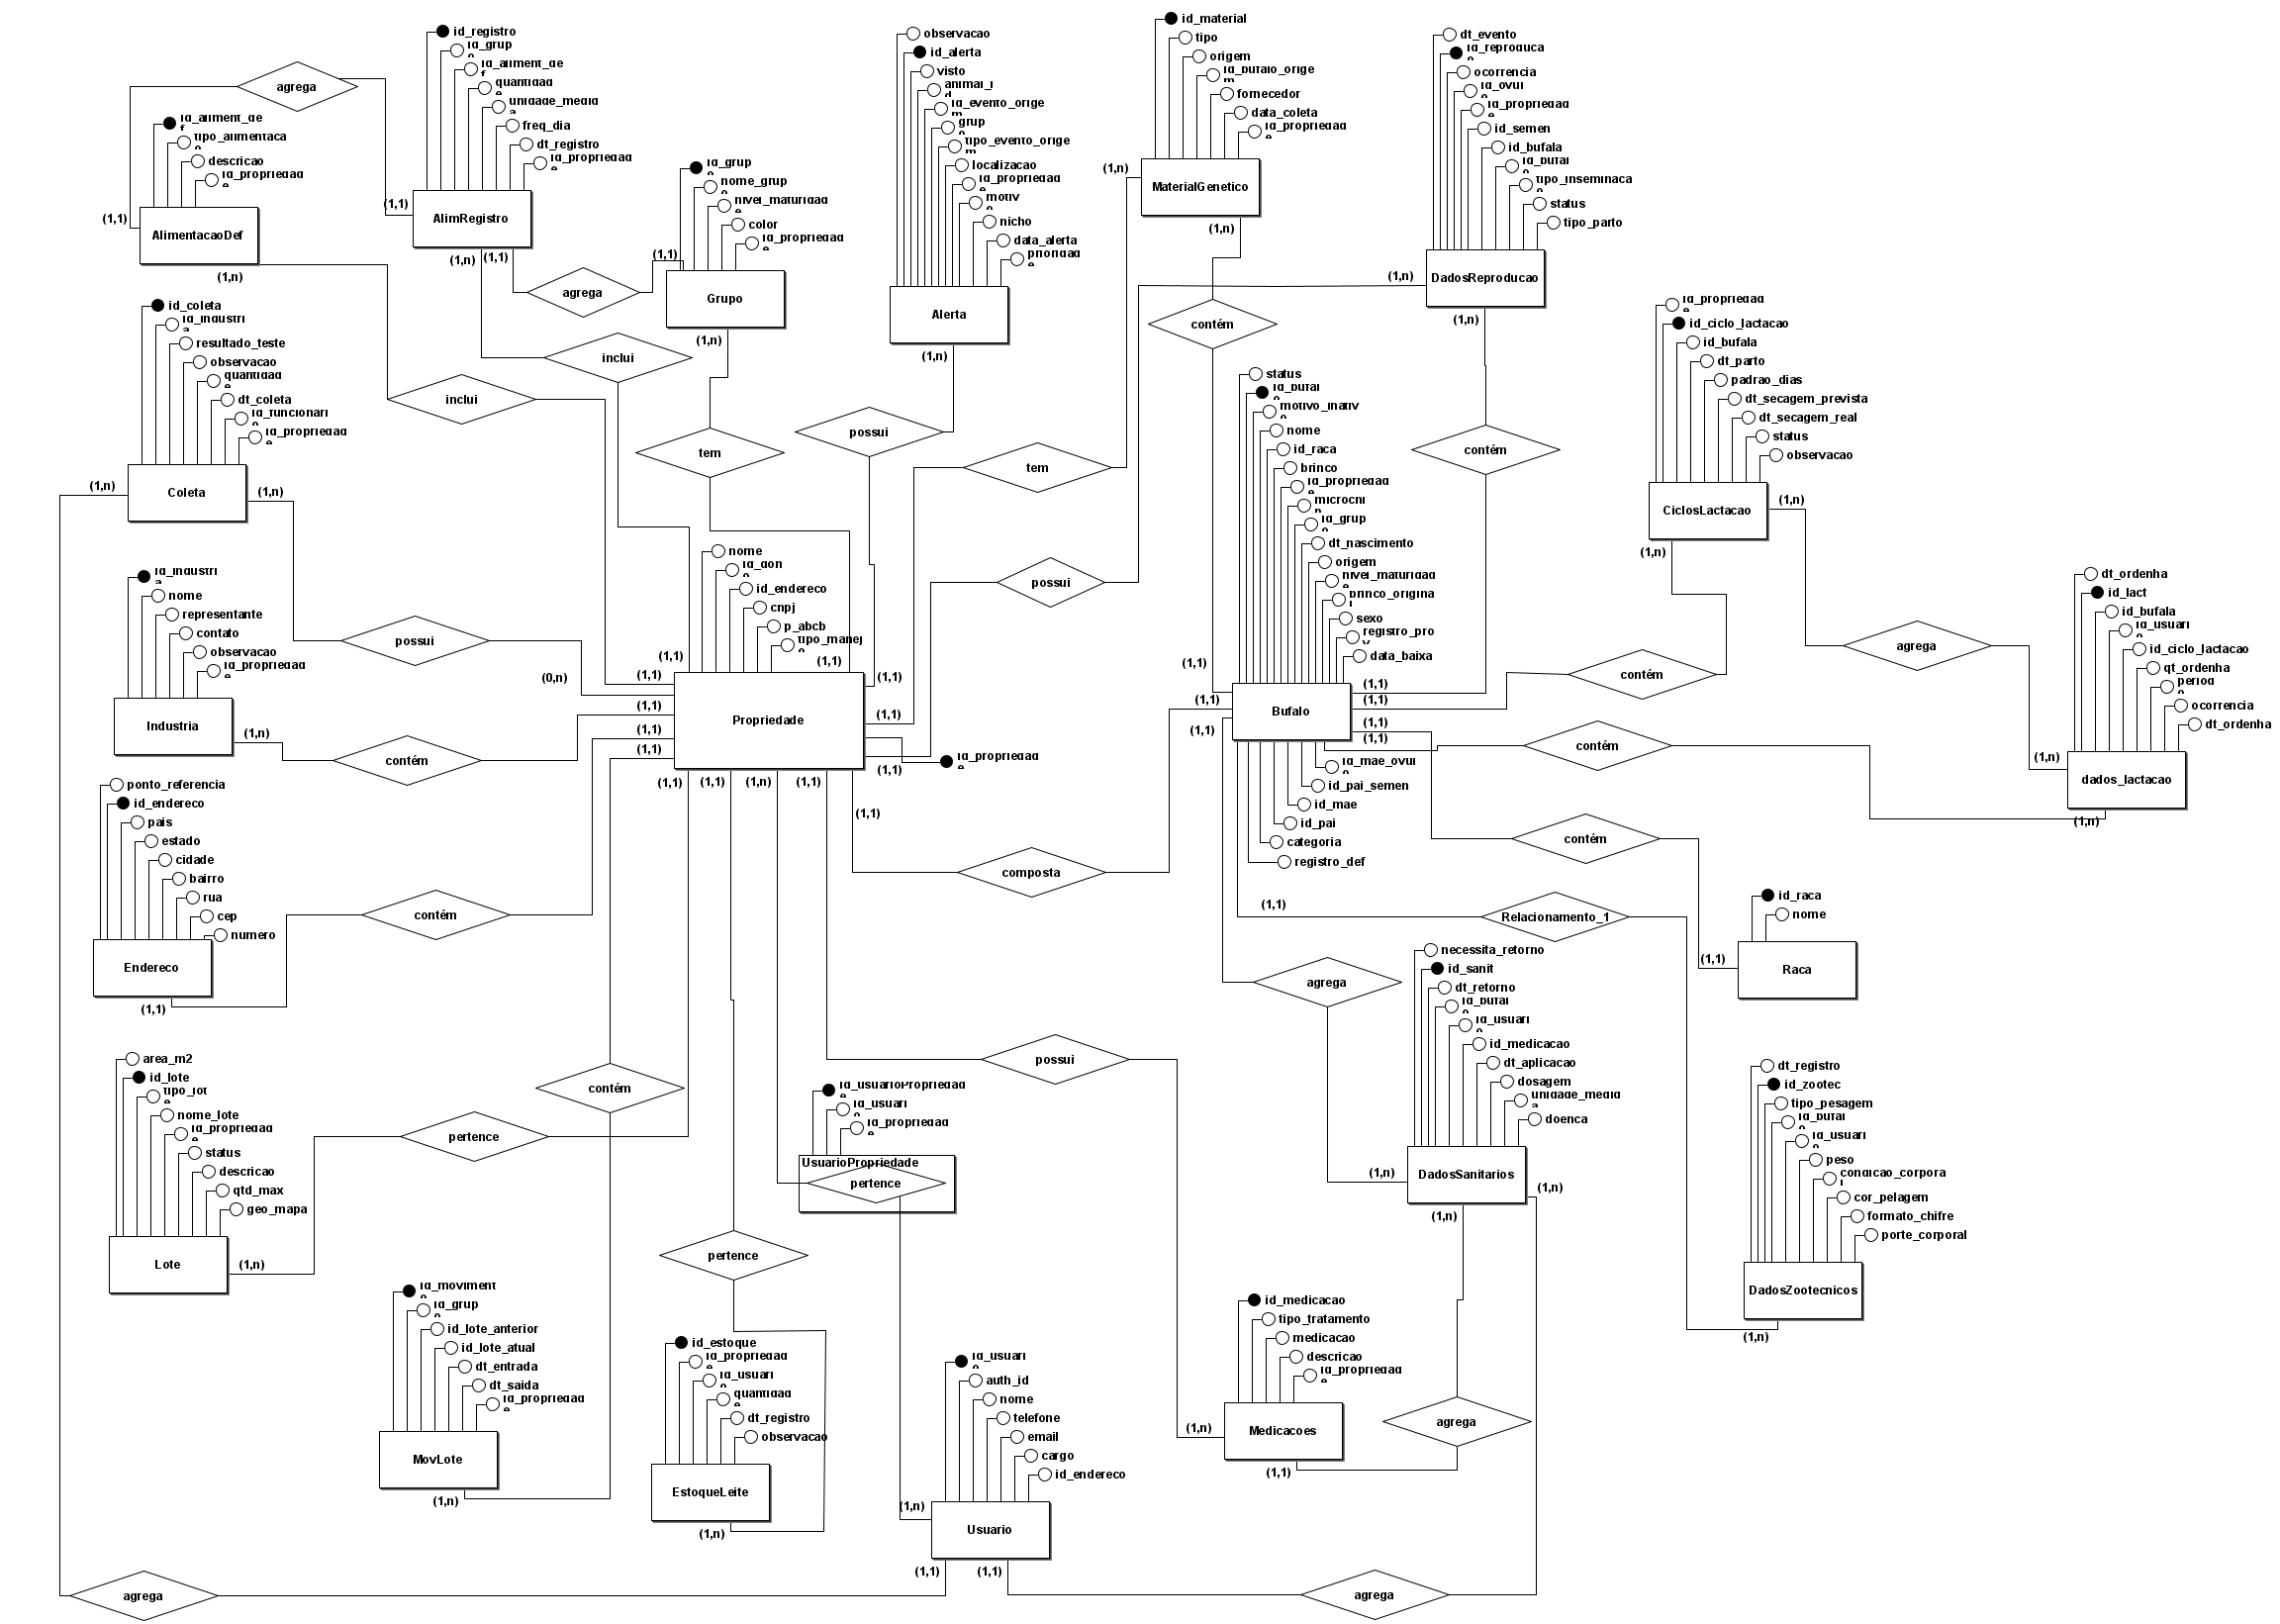
\includegraphics[width=1.1\textwidth]{Logos/Conceitual_buffs.png}
\SourceOrNote{Propria Autoria (2025)}
\end{figure}
De acordo com o avanço do projeto, o Modelo Banco de dados pode ser alterado.

\newpage
\section*{Modelo Lógico Banco de dados}
A seguir, é apresentado o modelo lógico do banco de dados, derivado do modelo conceitual. Nessa etapa, as entidades e relacionamentos são refinados em tabelas, chaves primárias e estrangeiras, garantindo a integridade referencial e a coerência dos dados conforme as regras de negócio do sistema.
\subsection*{Modelo Lógico Banco de dados}
 \addcontentsline{toc}{section}{Modelo Lógico Banco de dados}

     \begin{figure}[h]
\centering
\caption{Modelo Banco de dados}%
\label{fig:modelo-conceitual}
\includegraphics[width=1.1\textwidth]{Logos/Lógico_Buffs.png}
\SourceOrNote{Propria Autoria (2025)}
\end{figure}
De acordo com o avanço do projeto, o Modelo Banco de dados pode ser alterado.


\newpage
\section*{Desenvolvimento do Canvas}
Nesta seção será apresentado o Canvas utilizado para a modelagem do sistema desenvolvido. O Canvas detalha aspectos essenciais, como propostas de valor, segmentos de clientes, canais de distribuição, estrutura de custos e fontes de receita, servindo como uma ferramenta visual para organização e planejamento estratégico.
 \addcontentsline{toc}{section}{Canvas}
     \begin{figure}[h]
\centering
\caption{Canvas}%
\label{fig:canvas}
\includegraphics[width=0.8\textwidth]{Logos/Canvas.png}
\SourceOrNote{Propria Autoria (2025)}
\end{figure}

\newpage
\section*{Diagrama e Especificação da Infraestrutura da Rede}
Nesta seção é apresentada a arquitetura de rede e hospedagem do sistema desenvolvido. O ambiente foi estruturado de forma distribuída em serviços de nuvem, a fim de garantir escalabilidade, desempenho e disponibilidade. A API e o módulo de Inteligência Artificial foram hospedados em uma instância EC2 da AWS, responsável pelo processamento e integração com os demais componentes. O front-end web foi implantado na plataforma Vercel, permitindo a publicação e entrega contínua da interface do usuário. Já o banco de dados relacional PostgreSQL está hospedado no Supabase, que oferece gerenciamento, autenticação e acesso seguro aos dados do sistema.\addcontentsline{toc}{section}{Rede}
     \begin{figure}[h]
\centering
\caption{Rede}%
\label{fig:rede}
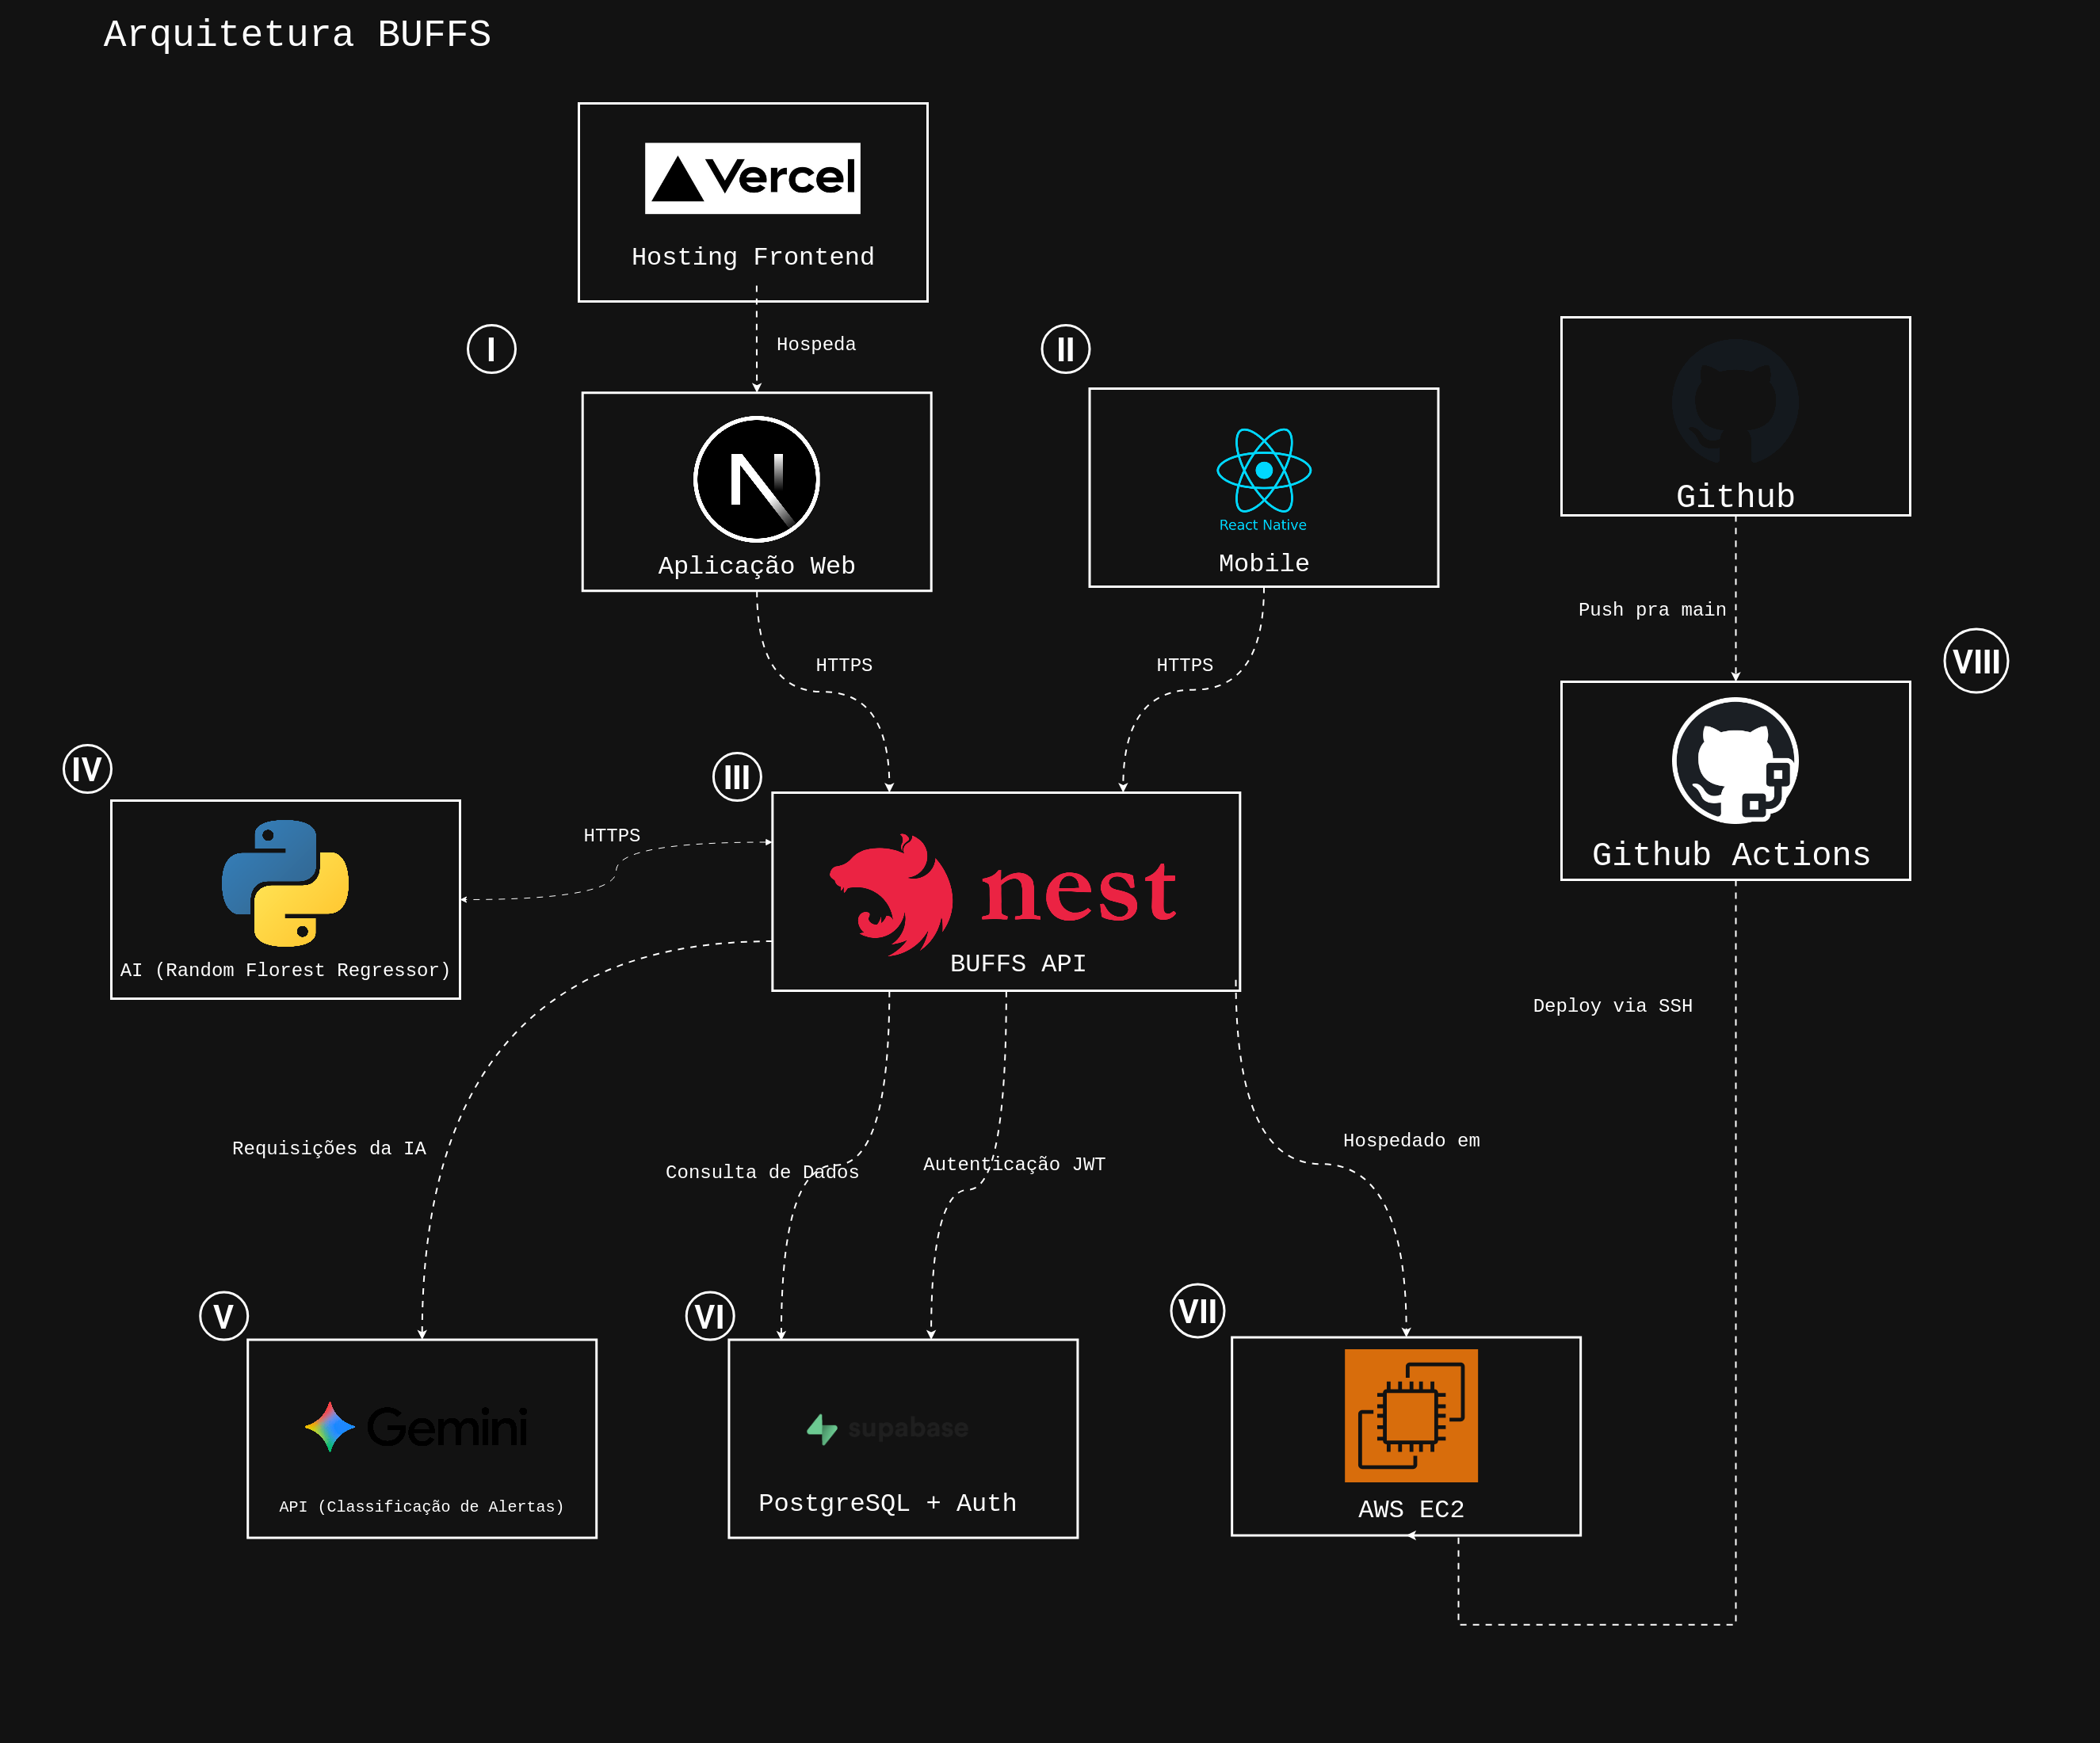
\includegraphics[width=0.9\textwidth]{Logos/buffs-arch-model.png}
\SourceOrNote{Propria Autoria (2025)}
\end{figure}

\newpage
\section*{Análise SWOT}
Nesta seção apresentamos a Análise SWOT do projeto, evidenciando pontos fortes (Strengths), fraquezas (Weaknesses), oportunidades (Opportunities) e ameaças (Threats). Cada quadrante fornece insights estratégicos que orientam decisões de desenvolvimento e implementação, ajudando a maximizar vantagens competitivas e mitigar riscos.
\addcontentsline{toc}{section}{Análise SWOT}

\begin{figure}[h]
  \centering
  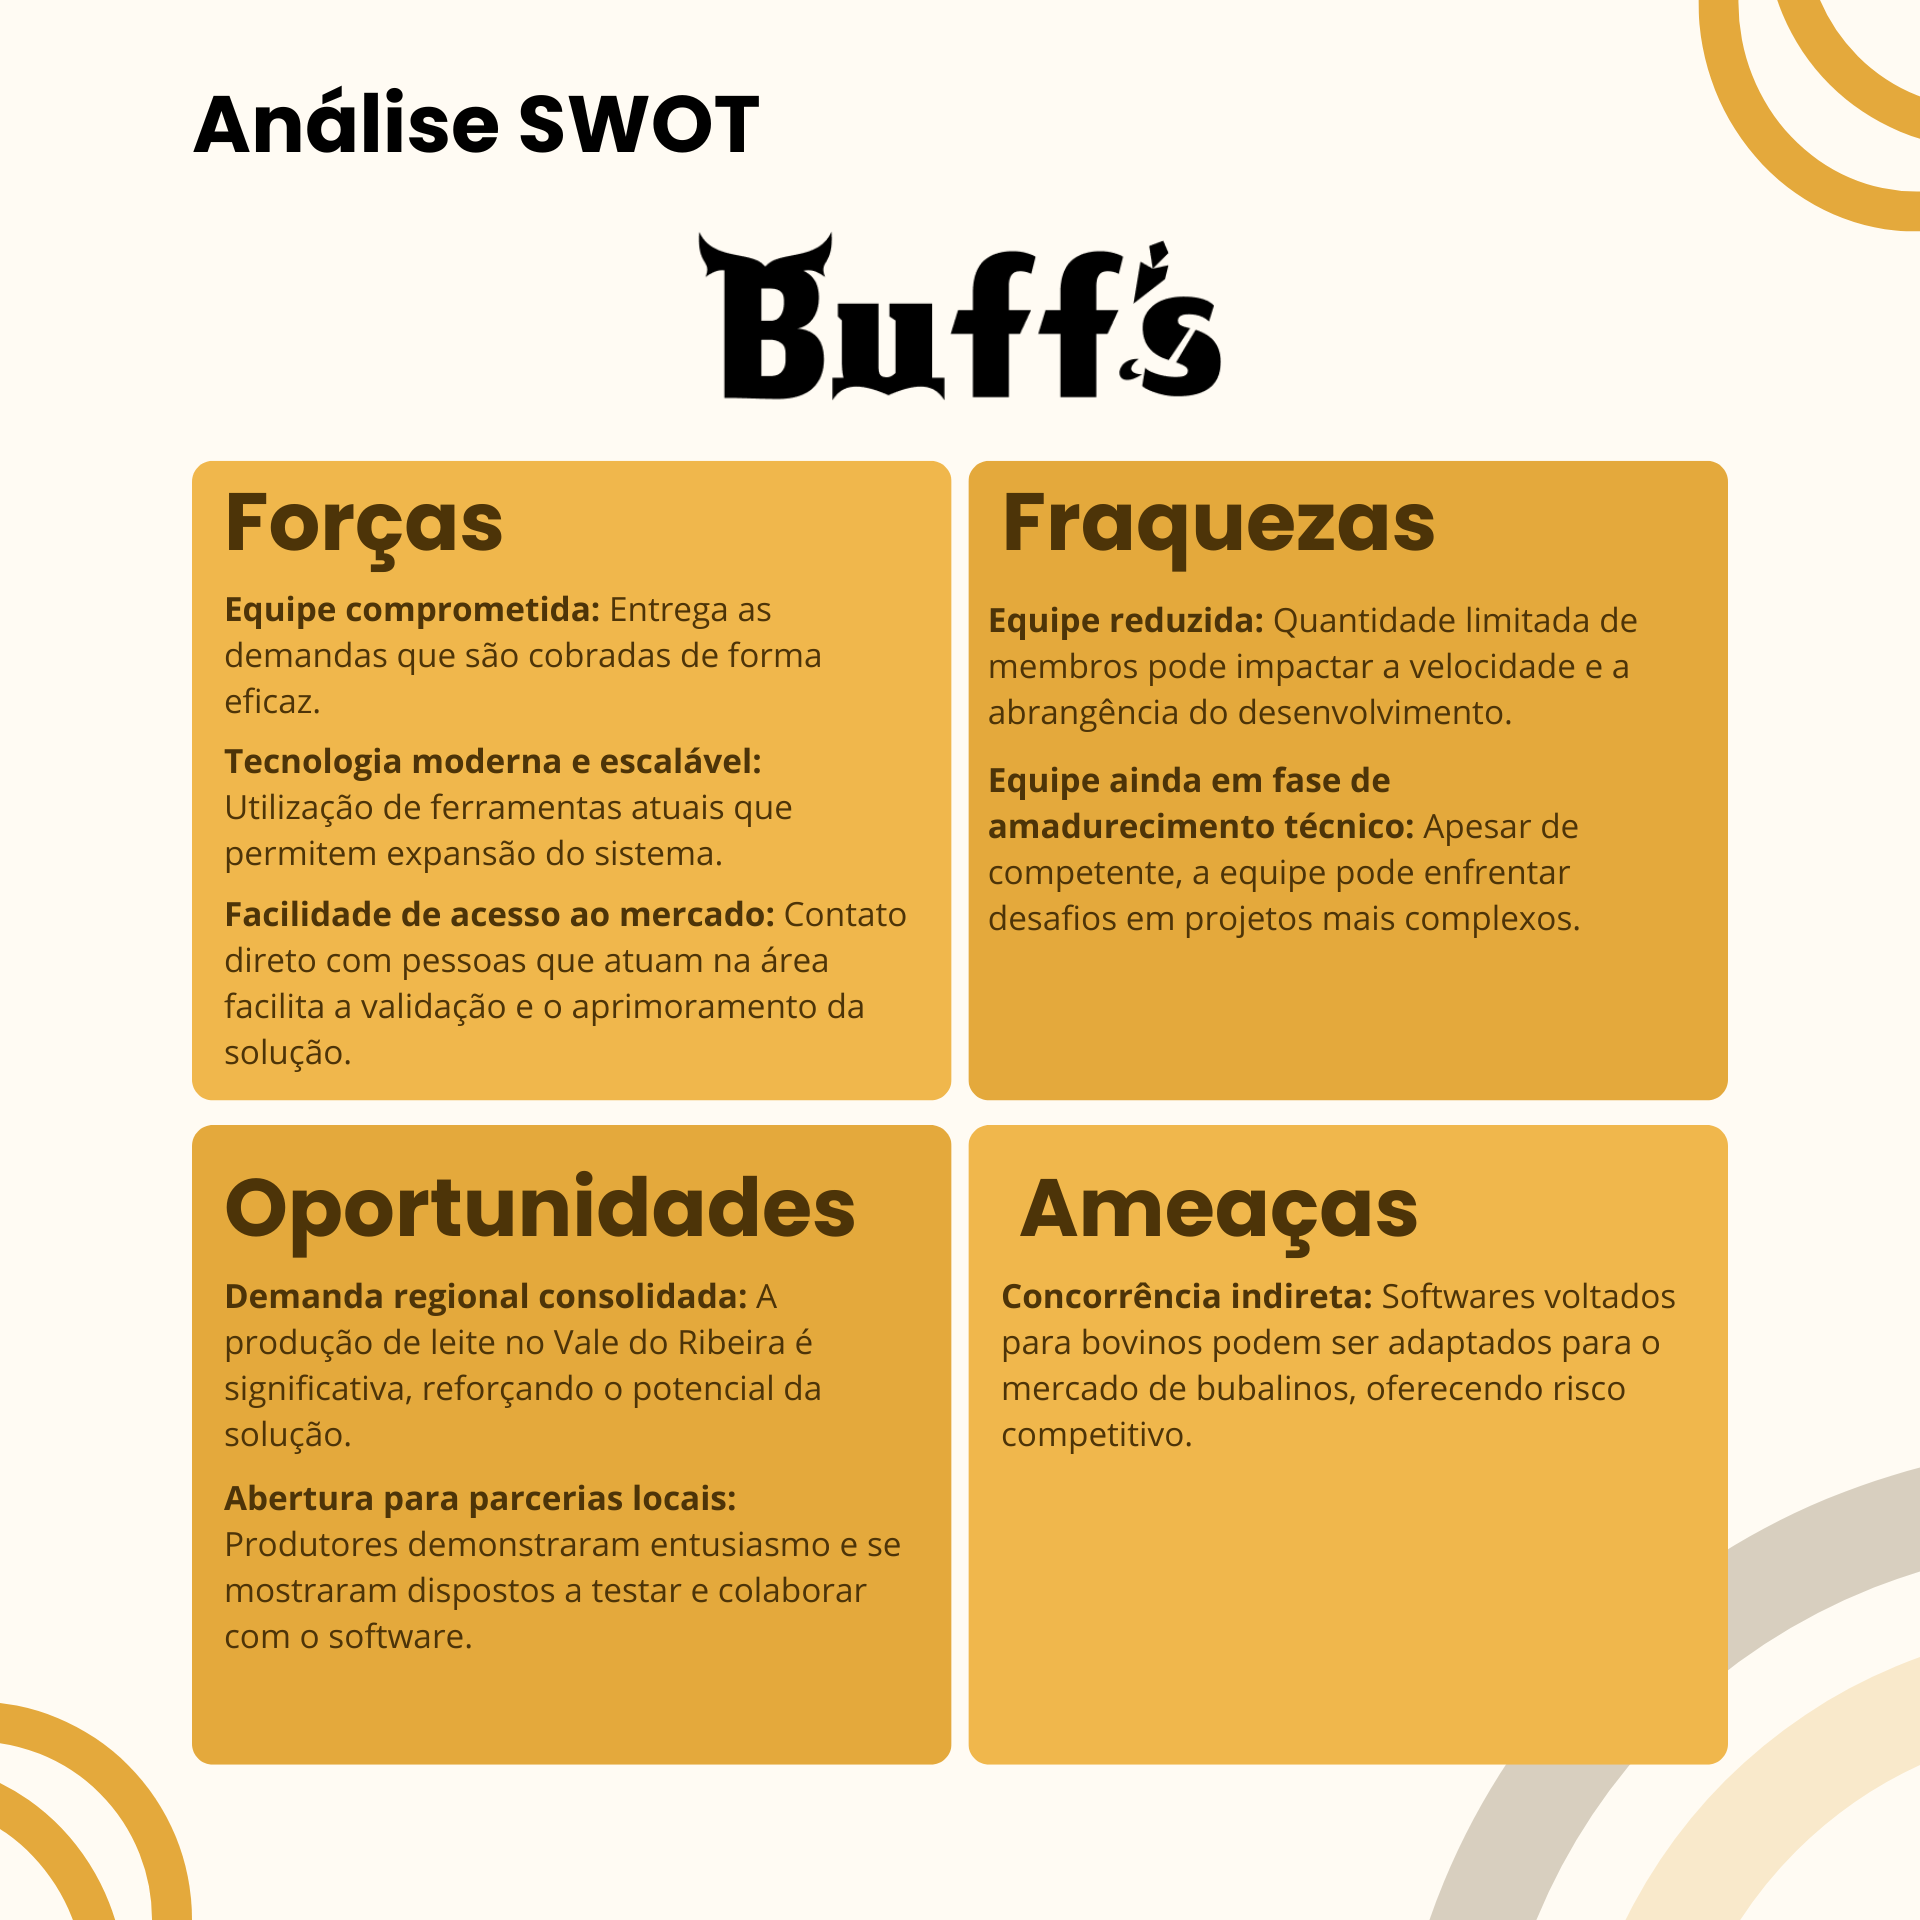
\includegraphics[width=0.8\textwidth]{Logos/SWOT.png}
  \label{fig:swot}
  \SourceOrNote{Própria autoria (2025)}
\end{figure}





\end{document}